\documentclass[a4paper,10pt]{article}
    %\documentclass[a4paper,10pt]{scrartcl}
    
    \usepackage[utf8]{inputenc}
    \usepackage{acro}
    \usepackage{float}
    \usepackage[portuguese]{babel}
    \usepackage{hyperref}
    
    \usepackage[colorinlistoftodos,prependcaption,textsize=tiny]{todonotes}
    \newcommand{\unsure}[1]{\todo[linecolor=red,backgroundcolor=red!25,bordercolor=red]{#1}}
    \newcommand{\change}[1]{\todo[linecolor=blue,backgroundcolor=blue!25,bordercolor=blue]{#1}}
    \newcommand{\info}[1]{\todo[linecolor=green,backgroundcolor=green!25,bordercolor=green]{#1}}
    \newcommand{\improvement}[1]{\todo[linecolor=blue,backgroundcolor=blue!25,bordercolor=blue]{#1}}
    \newcommand{\thiswillnotshow}[1]{\todo[disable]{#1}}
    
    \title{Desenvolvimento e Validação de Sistema para Eletrodiagnóstico Automático da Excitabilidade Neuromuscular}
    \author{Jonathan Ferreira Bispo}
    \date{}
    
    \pdfinfo{%
      /Title    ()
      /Author   ()
      /Creator  ()
      /Producer ()
      /Subject  ()
      /Keywords ()
    }
    
    \DeclareAcronym{tede} {
	short = TEDE,
	long = Teste de Eletrodiagnóstico de Estímulo,
	class = abbrev
}

\DeclareAcronym{cti} {
	short = CTI,
	long = Centro de Tratamento Intensivo,
	class = abbrev
}

\DeclareAcronym{eenm} {
	short = NMES,
	long =  Estimulação Elétrica Neuromuscular,
	class = abbrev
}

\DeclareAcronym{lm} {
	short = LM,
	long =  Lesão Medular,
	class = abbrev
}

\DeclareAcronym{asia} {
	short = ASIA,
	long =  American Spinal Injury Association,
	class = abbrev
}

\DeclareAcronym{icc} {
	short = ICC,
	long =  Intraclass Correlation Coefficient - Coeficiente de Correlação Intraclasse,
	class = abbrev
}

\DeclareAcronym{dac} {
	short = DAC,
	long =  Digital Analog Converter - Conversor Analógico Digital,
	class = abbrev
}
    
    \begin{document}
    
    \maketitle
    
    \section{Introdução}

O \ac{tede} é um exame não invasivo que detecta alterações de excitabilidade neuromuscular quantificando as respostas evocadas pelo nervo e pelo músculo com parâmetros de corrente elétrica, sendo composto pela mensuração da reobase, cronaxia e índice de acomodação \cite{sluga2002,schuhfired2005,lee2013}.

Em pacientes com \ac{lm}, a reabilitação requer o diagnóstico do nível e da gravidade da lesão por meio da identificação das zonas sensório-motoras íntegras, o que permite o tratamento e o prognóstico, bem como acompanhar a recuperação do sistema nervoso. Apesar da escala da \ac{asia} ser o método padronizado para essa avaliação \cite{van2011}, sua aplicação é limitada a pacientes não-cooperativos e ela não fornece todos os dados necessários para o entendimento de alterações fisiológicas e estruturais secundárias. Sendo assim, para este tipo de tratamento, os exames eletrofisiológicos que avaliam a condução nervosa são muito utilizados na busca por comprometimentos neuromusculares.

Pacientes que estejam há muito tempo sem mobilidade devido à, por exemplo, internação em \ac{cti} podem apresentar perda de massa muscular e atrofia.

Em todos os casos citados, terapias envolvendo \ac{eenm} são de grande valia para ajudar na avaliação, prevenção, diagnóstico ou melhoria na condição neuromuscular.

A eficiência do \ac{eenm} pode ser avaliada pelo torque causado devido à eletroestimulação artificial aplicada, sendo este torque diretamente relacionado à largura de pulso e amplitude dos estímulos.

Porém não existe concenso sobre os valores ideiais para tais parâmetros, sendo obtidos com base nos testes de reobase, cronaxia e índice de acomodação. 

A reobase é a menor intensidade de corrente com forma de pulso retangular e largura de pulso infinita para provocar contração muscular visível. A cronaxia é o menor tempo necessário para causar também contração muscular visível, com amplitude de corrente quadrada igual a duas vezes a reobase. A acomodação é a menor intensidade de corrente necessária para produzir contração muscular, mas com a forma de onda exponencial e largura de infinita, avaliando assim a capacidade do músculo em responder a altas intensidades e pulsos de crescimento lento. O índice de acomodação é a relação entre a acomodação e a reobase \cite{sluga2002}.

Apesar desses testes serem de grande importância, sua aplicabilidade clínica pode ser comprometida por serem operador-dependente e necessitarem de inspeção visual, podendo gerar falsos positivos ou falsos negativos, conferindo grande variabilidade aos testes.

Logo, ter um equipamento que possa tornar esses exames mais eficientes, rápidos e menos operador-dependente torna-se importante na aplicação clínica e acadêmica.
    \section{Objetivos}

\subsection{Objetivo Geral}
Desenvolver e validar um eletroestimulador multicanais automático com biofeedback para  substituir o eletrodiagnóstico manual feito atualmente com a mesma ou maior eficiência.
\subsection{Objetivos específicos}
\begin{itemize}
  \item Diminuir o tempo de execução dos exames.
  \item Aumentar a reprodutibilidade dos exames por meio da avaliação intra e inter observadores.’
  \item Identificar mais facilmente os pontos de maior excitabilidade muscular.
\end{itemize}
    \section{Materiais e métodos}

A eletroestimulação será feita pelo equipamento proposto no músculo tibial anterior da perna dominante. Entre os eletrodos será fixado um sensor acelerômetro para detectar a contração muscular por meio do circuito de biofeedback. Os eletrodos e o acelerômetro serão fixados com fita microporo e será adicionado gel condutor aos eletrodos para melhorar o contato com a pele. Será feita tricotomia na pele.

O sistema será dividido em quatro partes principais: Unidade de Controle, Unidade de Potência, Biofeedback e Interface Gráfica. A unidade de controle será responsável por gerar as formas de onda, em tempo real, por meio dos \ac{dac} de um microcontrolador. A unidade de potência alimentará todo o sistema fornecendo as tensões necessárias para os diversos componentes atuarem. Serão utilizadas fontes de corrente controladas por tensão para gerar os estímulos. O sistema de biofeedback será composto pelo acelerômetro utilizado para detectar a contração muscular. Um algoritmo que lê continuamente os eixos do acelerômetro será escrito para identificar alguma variação considerável em dua posição, detectando assim a contração muscular. A inteface gráfica com o usuário será um aplicativo Android que se comunicará via bluetooth com o eletroestimulador.

O eletroestimulador possuirá 12 canais, permitindo que 12 grupos musculares sejam estimulados simultamente. Para o presente trabalho, somente o músculo tibial anterior será eletroestimulado.

Serão feitos testes de bancada no equipamento, conectando uma carga de 1 $k\Omega$ para simular a resistência da pele. Um osciloscópio será utilizado para verificar se as formas de onda geradas bem como os valores máximos esperados estão sendo gerados pelo sistema.

Serão feitos exames por três avaliadores. Cada avaliador executará os exames de reobase e cronaxia convencionais, observando o músculo até notar a contração muscular, e de forma automática com o equipamento, efetuando teste e re-teste com os mesmos indivíduos com intervalo de dias a definir. O sistema será programado para não interromper automaticamente a eletroestimulação quando o avaliador estiver realizando o exame manual. Logo sem seguida, uma análise de \ac{icc} será conduzida para avaliar a variabilidade das observações entre diferentes observadores e do mesmo observador, comparando com os resultados obtidos pelo equipamento.

Para avaliação da reobase será utilizada uma onda retangular bifásica com largura de pulso de 1s fixa e 2s de descando, amplitude começando em 1 mA, sendo incrementada de 1 em 1 mA.

Para avaliar a cronaxia também será utilizada uma onda retangular bifásica porém com largura de pulso iniciando 20 $\mu$s incrementando de 20 em 20 $\mu$s, com 2s de descanso, amplitude de corrente fixa igual a 2 vezes o valor da reobase.

O tamanho da amostra será definido após um estudo piloto com 10 indivíduos, que tem por objetivo mensurar a variância inicial, e definir assim um N ótimo para um teste estatístico com 95\% de confiança e 80\% de poder.

Os participantes do estudo serão indivíduos, homens e mulheres entre 18 e 60 anos, sem histórico de \ac{den}, considerados saudáveis.

As coletas serão realizadas no \ac{leb} da \ac{ufmg}.

No presente trabalho não será avaliada a acomodação, pois ela possui o mesmo resultado aparente da reobase, mudando a resposta fisiológica ao estímulo, não alterando assim o resultado para validação do eletrodiagnóstico automático. A remoção da acomodação do estudo também diminuirá o tempo para execução do mesmo, tornando o estudo mais viável.

Os voluntários estarão sentados em uma cadeira com apoio para as costas com a perna dominante esticada sobre outra cadeira.

Os resultados obtidos pelo equipamento serão armazenados em arquivo CSV e enviados para um servidor central para posterior análise estatística.


    \section{Cronograma}

A execução do projeto respeitará o seguinte cronograma:

\begin{figure}[H]
	\centering
	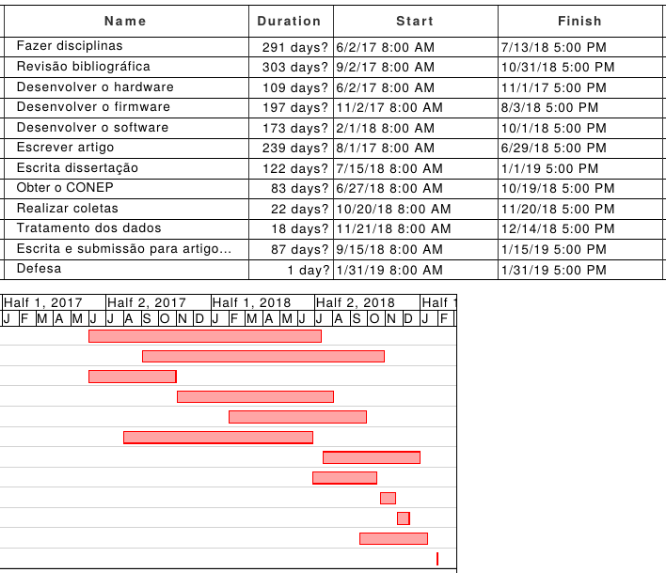
\includegraphics[width=1\textwidth]{cronograma/cronograma.png}
	\caption{Cronograma do Trabalho}
	\label{fig:cronograma}
\end{figure}
    \section{Expectativas}

Espera-se que o equipamento desenvolvido possa ser utilizado em \ac{uti} e clínicas para realização de \ac{tede}, tanto no setor público e privado. Sua aplicabilidade se estende também à pesquisa e inovação, podendo ser utilizado para realização de novos estudos sobre \ac{den}. Com potencial para ser utilizado também como ferramenta de terapia intensiva, futuramente o equipamento pode ser aplicado em \textit{home care}, trazendo o paciente que dependa de terapias intensivas para seu lar, criando assim um conforto para o mesmo, além de desonerar clínicas e hospitais que atualmente precisam manter este paciente por longos períodos de tempo em suas instalações.
    
    \bibliographystyle{unsrt}
    \bibliography{bibliografia}
    
    \end{document}
    